\section{Technical approach}
The main techniques for this problem can be described as follows
\begin{enumerate}
		\item \textbf{Face detection and landmark localization:} We employ dlib's face detection model, which utilizes Histogram of Oriented Gradients (HOG) features and a Support Vector Machine (SVM) classifier to locate faces in images. The system further identifies 68 facial landmarks corresponding to key facial features, establishing the foundation for emotion analysis.
		\item \textbf{Emotion classification:} We implement a Convolutional Neural Network (CNN) based on the ResNet-18 architecture to classify facial expressions into distinct emotional categories. We evaluate the model's performance against human benchmarks to validate its effectiveness, as emotion recognition is a challenging task even for humans.
\end{enumerate}
In this process, there may be some difficulties, especially in terms of efficiency. As the neural network is very computationally costly, we have to think of some methods to reduce time consumption.

The ways we thought of can be described as follows:
\subsection{Efficiency promotion}
\begin{enumerate}
    \item \textbf{Localized detection:} Since faces don't move much between frames, we track them by searching a small area around their last known spot. Only if a face goes missing do we scan the whole image again. Even if the scene suddenly shifts, we might miss just a single frame, no one would even notice.
    \item \textbf{Reduced resolution scanning:} To save computation during full-frame scanning, we lower the image resolution, as high detail isn't needed just to locate faces. For instance, using 480P instead of 1080P still allows accurate face detection while significantly reducing processing time.
    \item \textbf{Dynamic resolution adjustment:} when the face is very large, we can also reduce the resolution, as it is just about finding the face.
\end{enumerate}
\subsection{CNN recognition}
We observed that the data distribution was highly unbalanced. To address the imbalance in the dataset, especially the unde-rrepresentation of the disgust class, data augmentation was applied, leading to improved classification performance for rare emotions.

We employed a ResNet architecture for emotion classification. Facial expression classification is challenging even for humans. To establish a benchmark, we conducted experiments with our classmates. Initially, they achieved approximately 40\% accuracy, and even after extensive exposure to the dataset, their performance plateaued at around 60\%. Our model achieved an average test accuracy of 62\% (Figure \ref{fig:test_acc}), which is comparable to human performance.

\begin{figure}[!htb]
	\centering
	 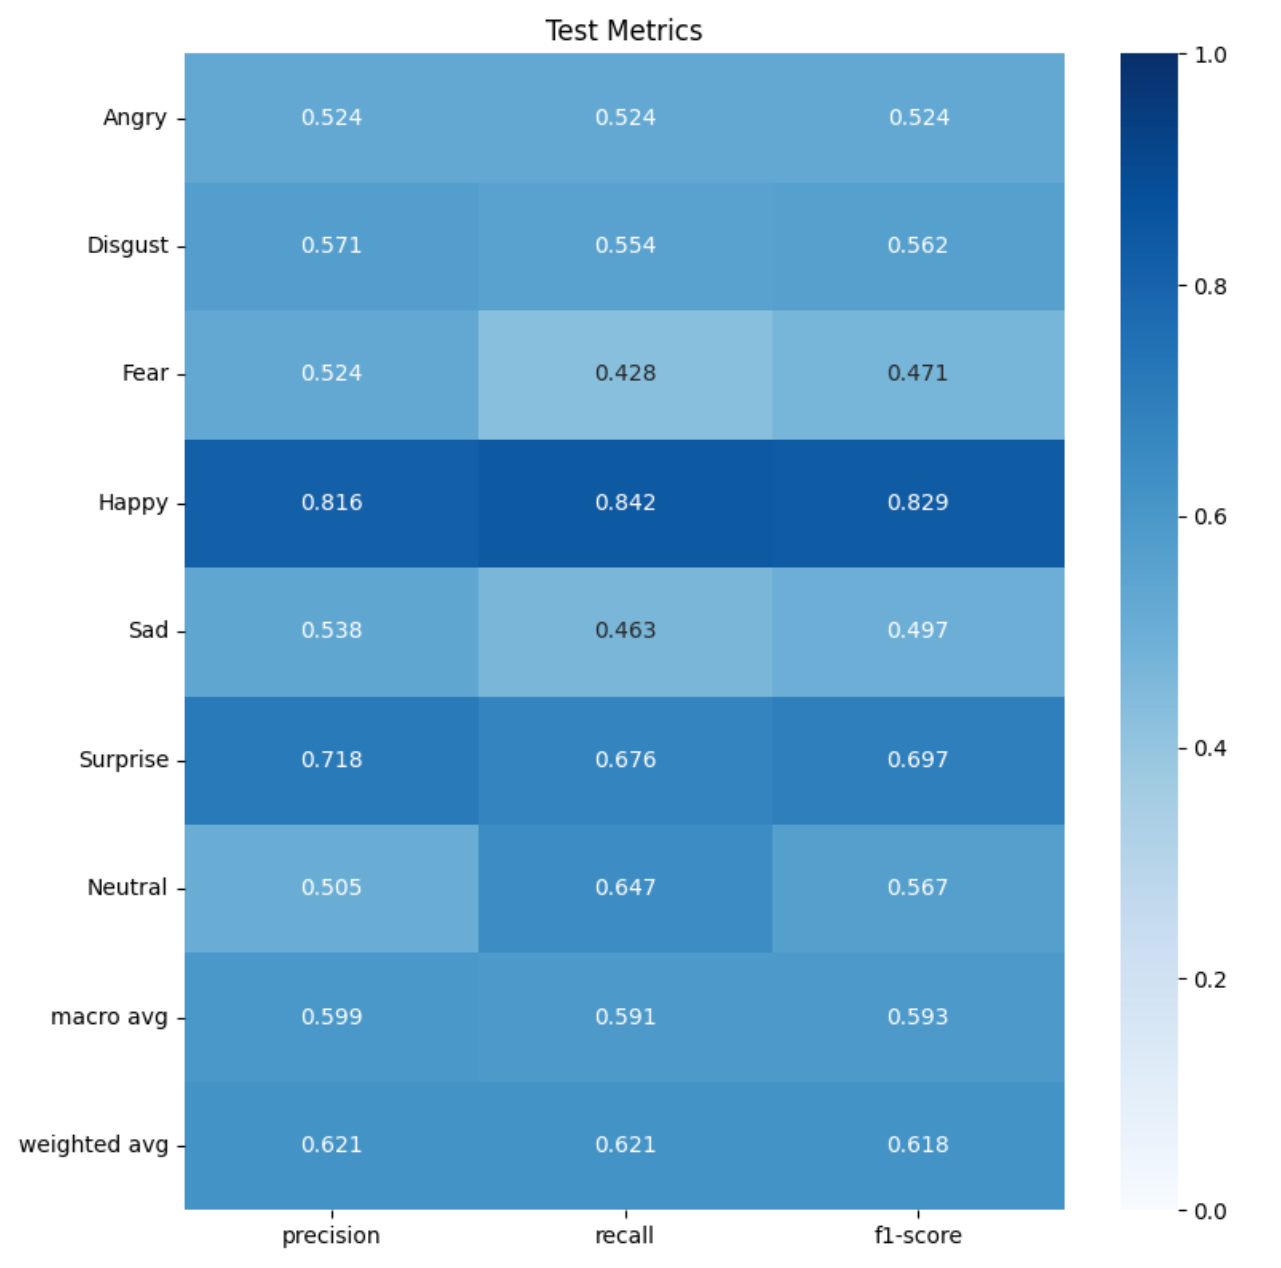
\includegraphics[width=0.6\linewidth]{sec/assets/test_acc.png}
	 \caption{The model achieved 62\% accuracy on the test set, comparable to trained human performance.}
	 \label{fig:test_acc}
\end{figure}

